\scanpage{22}
\textcircled{e}
\diagram{\begin{tikzcd}[row sep=large,column sep=large]
&\mathbb R\Gamma(W_0)\simeq\mathbb R\Gamma(Q)\simeq\mathbb R\Gamma(\mathring Q) \arrow[dl,dashed,"\beta'"']\\
{\begin{tikzpicture}[baseline=(current bounding box.center)]\node[draw,ellipse,inner sep=6pt] {$[\mathbb R\Gamma_!(\mathring P)]$};\end{tikzpicture}} \arrow[r,dashed] &\mathbb R\Gamma(W) \arrow[u,"\rho_1\ \text{compatible aux cup}"]
\end{tikzcd}}
\margin{\uline{NB} $\rho_1=\alpha\rho_0$\par\deleted{\unsure{a}}}

[Suite exacte de cohomologie relative pour $(W,W_0)$, ou $(W,Q)$, ou $(W,\mathring Q)$].

\uline{NB}. On a un hom \inserted{$(u_0,u_1,u_2)$} du triangle \textcircled{e} dans le triangle \textcircled{b}, \unsure{induit} par $(P,\partial P)\subset(W,Q\inserted{\unsure{W_0}\deleted{\unsure{W}}})$, avec
\[
u_1=\rho_0,\qquad u_2=\operatorname{inj}_1
\]
qui induit un isom $u_0$ qu'on aura à identifier \unsure{aux isos canons aux} $\unsure{\simeq|=}$ \unsure{objets} ....).
\margin{à \unsure{prouver} dans le cas algébrique; \unsure{donnera} \unsure{la justif. formelle} l'auto-dualité de $W$ et \unsure{une donnée de ce type} la donnée \textcircled{a'} plus bas}

\figure{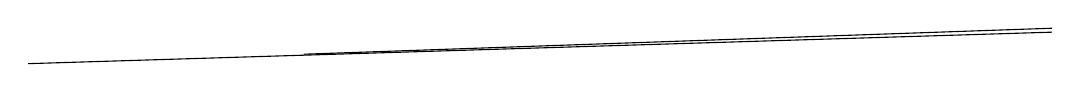
\begin{tikzpicture}\draw (0,0)--(13,.4);\draw (3.5,.12)--(13,.45);\end{tikzpicture}}

Supposons $W$ non singulière, i.e. $\mathring M$ non singulière, i.e. $\mathring P$ non singulière. Alors on a un isomorphisme
\[
\mathbb R(\Gamma,\pi)_!(\mathring M)\simeq\mathbb R\operatorname{Hom}_{\Lambda}\left(\underset{\substack{\Vert\\\mathbb R(\Gamma,\pi)(M)}}{K^\bullet},\Lambda\right)[-2n]
\]
et la flèche verticale de \textcircled{a} est une flèche
\diagram{\begin{tikzcd}[column sep=large]
\boxed{u:\ \mathbb R\operatorname{Hom}_{\Lambda}(K^\bullet,\Lambda)[-2n]\longrightarrow K^\bullet}&\text{dans }\mathrm D(\Lambda[\pi])
\end{tikzcd}}
i.e. un élément de
\[
\deleted{\unsure{\mathbb R\Gamma(\Lambda)}}\ H^{2n}(K^\bullet\overset{\mathrm L}{\otimes}_{\Lambda}K^\bullet)
\]
La donnée fondamentale \textcircled{a} devient
\textcircled{a'}
\diagram{\begin{tikzcd}[row sep=large,column sep=large]
& L^{\bullet\,\mathrm{triv}} \arrow[dl,"\rho'"']\\
\mathbb R\operatorname{Hom}_{\Lambda}(K^\bullet,\Lambda)[-2n] \arrow[r,very thick] &K^\bullet \arrow[u,"\rho"]
\end{tikzcd}}
\margin{$K^\bullet\in\operatorname{ob}\mathrm D(\Lambda[\pi])$;\par
$L^\bullet\in\operatorname{ob}\mathrm D(\Lambda)$\par
$K^\bullet$ parfait rel. à $\Lambda$}

En fait, $\rho$ et $\rho'$ \uuline{sont transposés} \uline{l'un de l'autre} (signe ?)
\mspage{21}
